\subsection{Backend des Web-Editors}\label{subsec:backend}
Das folgende Kapitel beschäftigt sich mit dem zweiten Bestandteil des Web-Editors, das Backend.
Vom Frontend wird eine YAML-Beschreibung an das Backend geschickt, in diesem wird dies als Eingabe für fulibWorkflows verwendet.
Da fulibWorkflows eine Java-Bibliothek ist, wird ein Backend benötigt, welches auf Java basiert.

\subsubsection{Spring Boot}
Mittels \textit{Spring Boot} ist es möglich ohne zusätzliche Konfiguration eine auf \textit{Spring} basierende Applikation zu erstellen\cite*{springBoot}.
Spring ist ein Framework, welches sich als Ziel gesetzt hat ``Java-Programmierung zu vereinfachen und zu verschnellern, allerdings keine Einbußen
bei Geschwindigkeit, Komplexität und Produktivität zu machen''\cite*{spring}.
In diesem Kapitel wird sich mit der Erstellung eines \ac{REST}-Services befasst.
Ein \ac{REST}-Service stellt Endpunkte bereit, welche über \ac{REST} angesprochen werden können.
Diese eignen sich zur Nutzung als simples Backend.

\begin{figure}[h]
    \centering
    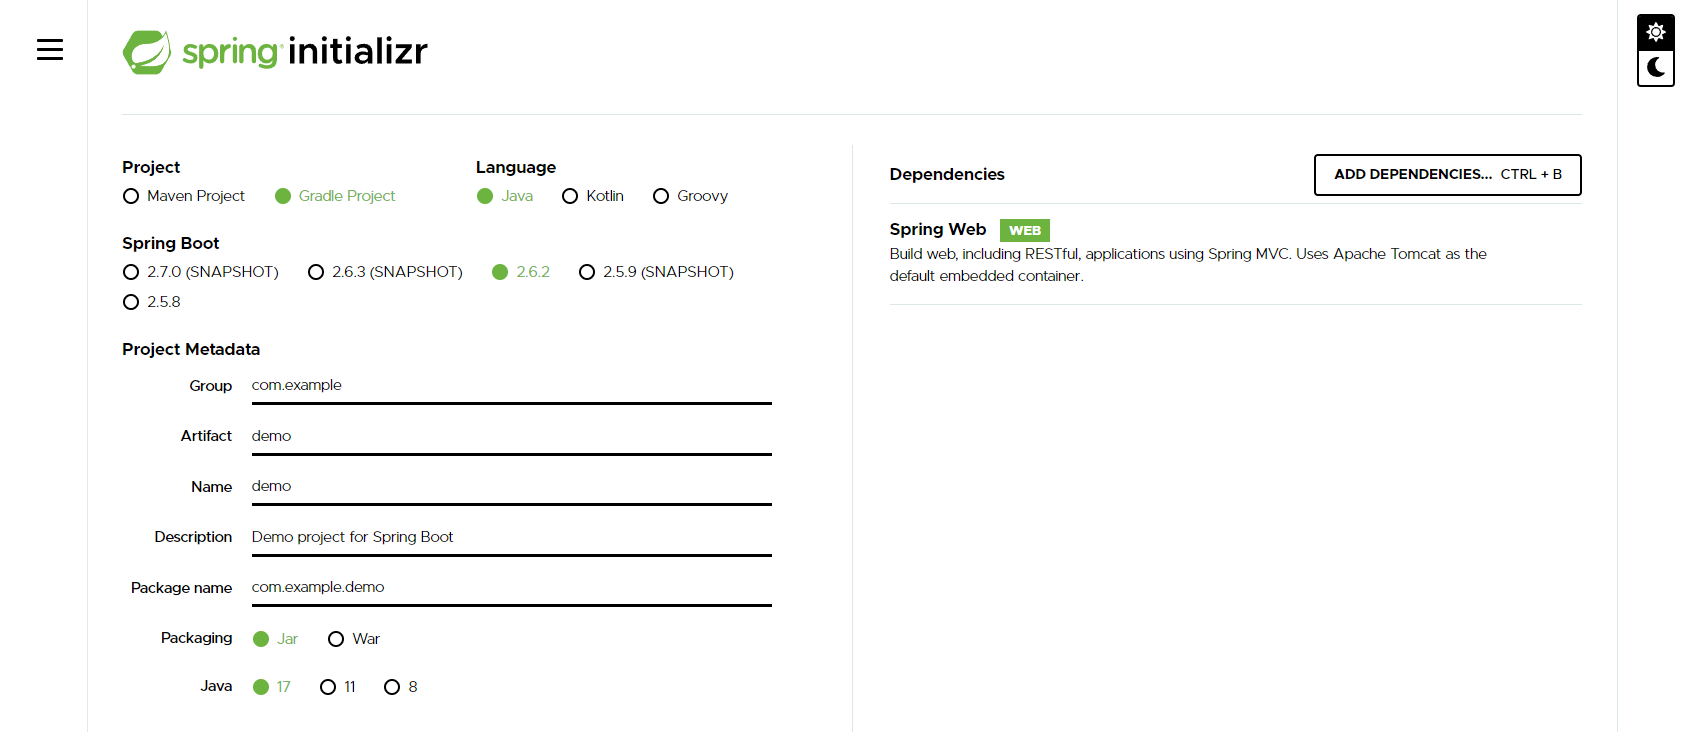
\includegraphics[width=1.0\textwidth]{images/2.2/spring-init}
    \caption{Spring Initializr für eine Web-Anwendung}
    \label{fig:spring-init}
\end{figure}


Das Anlegen eines Spring-Boot-Projektes kann durch den \textit{Spring Initializr} erledigt werden, dabei handelt es sich um eine Webseite, welche in
Abbildung~\ref{fig:spring-init} zu sehen ist\cite*{sbinit}.
Hierbei können diverse Einstellungen getätigt werden, um das zu generierende Projekt an die Anforderungen des Benutzenden anzupassen.
Die Abbildung zeigt die getätigten Einstellungen, um ein Gradle-Projekt mit Java-Version 17 als Programmiersprache zu generieren.
Ebenfalls kann die Version von Spring Boot eingestellt werden.
Zusätzliche Dependencies können im rechten Bereich des \textit{Spring Initializrs} hinzugefügt werden.
In diesem Fall wurde \textbf{Spring Web} ausgewählt, wodurch die wichtigsten Dependencies für eine \ac{REST}-Applikation bereits enthalten sind.

Das mit diesen Einstellungen generierte Projekt ist bereits ein fertiges Backend, welches direkt ausgeführt werden kann.
Durch sogenannte Annotations können weitere Endpunkte hinzugefügt werden.
In Kapitel~\ref{sec:editor-backend} werden Beispiele hierzu gezeigt und erläutert.
Auf die genaueren Funktionen, welche mittels Annotations implementiert werden können, wird in Kapitel~\ref{sec:editor-backend} eingegangen, anhand von Beispielen der Implementierung.

